\documentclass[10pt]{beamer}

\usetheme{glasgow}

\usepackage{booktabs}
\usepackage[scale=2]{ccicons}
\usepackage{minted}
\usepackage{bookmark}
% \sisetup{per-mode=symbol,per-symbol = p}
\usepackage[style=verbose]{biblatex}
\renewcommand{\footnotesize}{\fontsize{5pt}{7pt}\selectfont}
% \usepackage{filecontents}% to embed the file `myreferences.bib` in your `.tex` file
% \begin{filecontents*}[noheader]{references.bib}
%     @book{rappaport_millimeter_2015,
% 	address = {Upper Saddle River, NJ},
% 	title = {Millimeter wave wireless communications},
% 	isbn = {978-0-13-217228-8},
% 	publisher = {Prentice Hall},
% 	author = {Rappaport, Theodore S. and Heath, Robert W. and Daniels, Robert C. and Murdock, James N.},
% 	year = {2015},
% 	keywords = {Millimeter wave communication systems, Wireless communication systems}
% }

% \addbibresource{references.bib}


% \usepackage[noadjust]{cite}
\usepgfplotslibrary{dateplot}

\usemintedstyle{trac}

% ($ (A)!r!(B) $) the location of images to be used
\graphicspath{{src/}}

%% Customisation
% \newcommand{\V}[1]{\v} % vectors \v{c}
% \renewcommand{\v}[1]{\mathbf{#1}} % vectors
\newcommand{\ti}[1]{\tilde{#1}} % spectral representation
\newcommand{\tnsr}[1]{\underline{\underline{#1}}}

% Symbols
\renewcommand{\O}{\omega}  % omega
\newcommand{\E}{\varepsilon}  % epsilon
\renewcommand{\u}{\mu}  % mu
\newcommand{\p}{\rho}  % rho
\newcommand{\x}{\times}  % times
\renewcommand{\inf}{\infty}  % infinity
\newcommand{\infint}{\int\limits_{-\inf}^\inf} % integral by R
\newcommand{\e}{\mathrm{e}} % Straight-up exponential
\renewcommand{\j}{{j}\mkern1mu} % Straight-up exponential
\newcommand{\iu}{\mathrm{i}\mkern1mu}

\newcommand\ddfrac[2]{\frac{\displaystyle #1}{\displaystyle #2}}

\usepackage{animate}



%     % Define a the counter cnt. Used to identify files generated for use
% % with Gnuplot.
% \newcounter{cnt}
% \setcounter{cnt}{0}

% % Macro for drawing one frame of the F-distribution animation.
% \newcommand{\fdst}[4]{%
%     % shade the critical region tail
%     \draw[fill,orange]  (#1,0) -- plot[id=5\thecnt,domain=#1:5.5,samples=50]
%         function {#4*(x**(0.5*#2-1))*((1+#2*x/#3)**(-0.5*#2-0.5*#3))}
%             -- (5.5,0) -- cycle;

%     % draw the F distribution curve
%     \draw[color=blue!50!black,thick]
%         plot[id=f4\thecnt,smooth,domain=0:5.5,samples=100]
%         function {#4*(x**(0.5*#2-1))*((1+#2*x/#3)**(-0.5*#2-0.5*#3))};

%     % draw the F axis
%     \draw[->] (0,0) -- (6,0) node[right] {$F$};
%     % label the critical region boundary
%     \draw (#1,0) -- (#1,-0.02) node[below] {$#1$};
%     % label 0
%     \draw (0,0) -- (0,-0.02) node[below] {$0$};

%     % add some lables for degrees of freedom and alpha level
%     \draw (2,0.5) node[right] {$df_1 = #2$};
%     \draw (2,0.4) node[right] {$df_2 = #3$};
%     \draw (2,0.3) node[right] {$\alpha = 0.10$};

%     % draw the y axis
%     \draw[very thin,->] (0,0) -- (0,0.8);
% }


\title{High Frequency Communication Systems}
\subtitle{Lecture 12 - Finishing it off\dots}
\date{Spring 2023}
\author{Hasan T Abbas \& Qammer H Abbasi}
% \institute{}





\begin{document}

\maketitle


% \begin{frame}
%     \frametitle{Course Evaluation Survey}

%     \begin{figure}[h!]
%         \centering
%         \includegraphics[width=.5\textwidth]{QRCode for High-Frequency Communication Systems.png}
%         \caption{Survey available at https://forms.office.com/r/uzegCvGdPE.}
%     \end{figure}
% \end{frame}

%%%%%%%%%%%%%%%%%%%%%%%%%%%%%%%%%%%%%%%%%%
%%%%%%%%%%%%%%%%%%%%%%%%%%%%%%%%%%%%%%%%%%
%%%%%%%%%%%%%%%%%%%%%%%%%%%%%%%%%%%%%%%%%%
\begin{frame}[fragile]
    \frametitle{Lecture Outline}
    \begin{outline}[itemize]
        \1 Going the extra mile
        \1 Disaggregation
        \1 Thoughts \dots
    \end{outline}
\end{frame}
%%%%%%%%%%%%%%%%%%%%%%%%%%%%%%%%%%%%%%%%%%
%%%%%%%%%%%%%%%%%%%%%%%%%%%%%%%%%%%%%%%%%%
%%%%%%%%%%%%%%%%%%%%%%%%%%%%%%%%%%%%%%%%%%

\begin{frame}
    \begin{figure}
        \includegraphics[height = 1.5in]{QRCode.png}
    \end{figure}
\end{frame}


\section{Metasurfaces}
\begin{frame}
    \frametitle{Wavefront Shaping.}

    \begin{columns} % align columns
        \begin{column}{.5\textwidth}
            \begin{minipage}[T][.1\textheight][c]{\linewidth}
                \begin{outline}[itemize]
                    \1 Mould the shape of a wavefront
                    \1 Challenge — Below optical frequencies, the EM wave loses its coherence when we move away from the source
                \end{outline}
            \end{minipage}
        \end{column}
        %
        \begin{column}{.5\textwidth}
            % Use this to preserve fonts from Inkspace
            \begin{figure}
                \includegraphics[height = 1.5in]{Metasurface.jpeg}
                \label{fig:cond_2deg}
                \caption{A metasurface illustration, from \tiny{[Achouri, Karim and Caloz, Christophe. Nanophotonics, vol. 7, no. 6, 2018]}.}
            \end{figure}
            %
        \end{column}%
    \end{columns}
\end{frame}


\begin{frame}
    \frametitle{A Phase Control Approach}

    \begin{columns} % align columns
        \begin{column}{.5\textwidth}
            \begin{minipage}[T][.1\textheight][c]{\linewidth}
                \begin{outline}[itemize]
                    \1 Mould the shape of a wavefront
                    \1 Challenge — Below optical frequencies, the EM wave loses its coherence when we move away from the source
                \end{outline}
            \end{minipage}
        \end{column}
        %
        \begin{column}{.5\textwidth}
            % Use this to preserve fonts from Inkspace
            \begin{figure}
                \includegraphics[height = 1.5in]{pr_meta.png}
                \label{fig:cond_2deg}
                \caption{Programmable Metasurface, from \tiny{[Zhang, L., Chen, X.Q., Liu, S. et al. Nat Commun 9, 4334 (2018)]}.}
            \end{figure}
            %
        \end{column}%
    \end{columns}
\end{frame}

\section{Terahertz Applications}

\begin{frame}
    \frametitle{Terahertz Detection}
    Relying on the principle of reciprocity, we can use photoconductive antennas to detect THz radiation.
    \begin{figure}[h!]
        \centering
        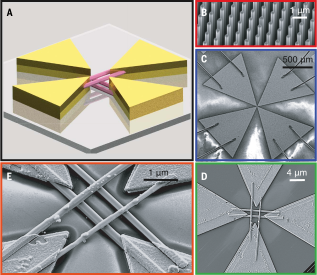
\includegraphics[width=.45\textwidth]{terahertz_applications.pdf}
        \caption{A polarisation sensitive cross-nanowire THz detector \tiny{[Peng et al., Science 368, 510-513 (2020)]}.}
    \end{figure}
\end{frame}

\begin{frame}
    \frametitle{Terahertz Imaging}
    \begin{outline}
        \1 THz waves have the ability to \textcolor{red}{see through} apparently opaque objects.
        \1 This is done in a non-ionising manner
        \1 Through image processing, we can achieve high-resolution imaging through THz waves.
    \end{outline}
    \begin{figure}[h!]
        \centering
        \includegraphics[width=.95\textwidth]{terahertz_imagin.png}
    \end{figure}
\end{frame}


\begin{frame}
    \frametitle{Material Characterisation}

    \small
    \begin{columns}
        \begin{column}{.4\textwidth}
            \begin{outline}
                \1 THz time-domain spectroscopy (THz-TDS) is a well-known method for charaterising the material properties of different substances
                \2 Attractive applications in explosives detection, counterfeit drug discovery and health monitoring of plants
                \1 The Biggest feature is again, the non-ionising nature of THz waves
                \1 Common substances such as \ch{H2O} and \ch{N2} have strong absorption spectra
             \end{outline}
        \end{column}
        \begin{column}{.6\textwidth}
            \scriptsize
            \begin{figure}[T!]
                \centering
                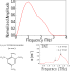
\includegraphics[width=.95\textwidth]{nitrogen.pdf}
                \label{fig:nitrogen}
            \end{figure}
        \end{column}
    \end{columns}
\end{frame}

\section{Software Defined Radio}

\begin{frame}
    \frametitle{Software Defined Radio - Motivation}
    \begin{outline}
    \1 A communication system consists of many layers of operations.
    \1 The physical layer is the most important of all.
    \1 Typically, physical layer processing is done via dedicated hardware
    \1 Radio is the technology through which signals are wirelessly transmitted and received
    \1 Software-defined radio has some or all physical layer functions implemented via software
\end{outline}
\end{frame}

\begin{frame}
    \frametitle{Software Defined Radio}
\begin{figure}[h!]
    \centering
    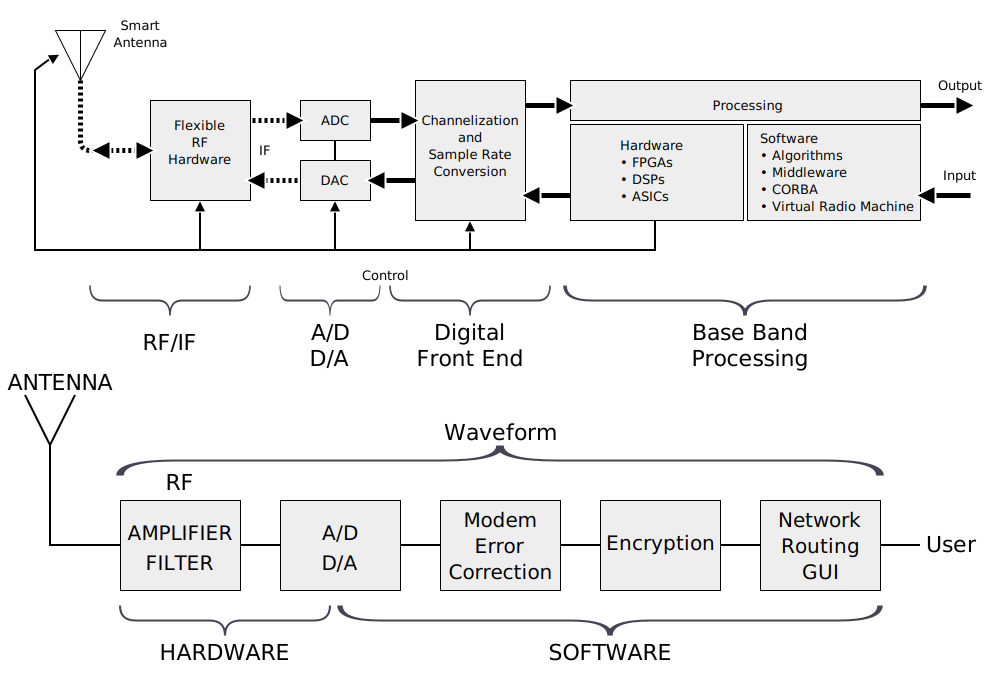
\includegraphics[width=.8\textwidth]{SDR_et_WF.pdf}
    \caption{A Typical SDR workflow}
\end{figure}
\end{frame}

\begin{frame}
    \frametitle{GNU Radio}
    \begin{columns}[] % align columns
        \begin{column}{.5\textwidth}
        \begin{outline}
            \small
    \1 A graphical user interface consisting of \textit{flowgraphs} through which different signal processing functions such as analogue-digital conversion can be performed.
    \1 Some additions let us write \texttt{Python} codes within each block
    \1 The software is meant to interface with Universal Software Radio Peripheral (USRP) modules to construct a complete communication system.
\end{outline}   
\end{column}
\begin{column}{.5\textwidth}
\begin{figure}[h!]
    \centering
    \includegraphics[width=.95\textwidth]{FSK_example_fg.png}
    \caption{GNU Radio Interface.}
\end{figure}
\end{column}%
\end{columns}   

\end{frame}


\end{document}
